\documentclass{report}

\usepackage{lipsum}
% Geometry and layout
\usepackage[margin=3.3cm]{geometry}
\usepackage[skip=10pt plus1pt, indent=0em]{parskip}
\usepackage{multicol}
\usepackage{titlesec}
\usepackage{csquotes}
\usepackage{float}
\usepackage{palatino}

\usepackage{fancyhdr}

% Links and references
\usepackage{hyperref}

% Math and symbols
\usepackage{amsmath}
\usepackage{amssymb}
\usepackage{amsthm}

% Graphics
\usepackage{graphicx}
\usepackage{svg}
\usepackage{tikz}

% Code listings
\usepackage{listings}
\usepackage{color}
\definecolor{dkgreen}{rgb}{0,0.6,0}
\definecolor{gray}{rgb}{0.5,0.5,0.5}
\definecolor{mauve}{rgb}{0.58,0,0.82}
\lstdefinestyle{mystyle}{
    aboveskip=3mm,
    belowskip=3mm,
    showstringspaces=false,
    columns=flexible,
    basicstyle={\small\ttfamily},
    numbers=left,
    numberstyle=\tiny\color{gray},
    keywordstyle=\color{blue},
    commentstyle=\color{dkgreen},
    stringstyle=\color{mauve},
    breaklines=true,
    breakatwhitespace=true,
    tabsize=3,
    xleftmargin=1em
}

\lstset{style=mystyle}

\usepackage{sourcecodepro}
\usepackage[T1]{fontenc}
\lstset{basicstyle=\ttfamily}

% Frames and boxes
\usepackage{mdframed}

% Theorems and remarks
\newtheorem*{remark}{Remark}

% Text
\makeatletter
\renewcommand\maketitle{
    \begin{center}
        \vspace*{12em}
        {\textbf{\LARGE{\@title}}} \\
        \vspace{1em}
        {\textbf{\Large{\@author}}} \\
        \vspace{1em}
        {\textbf{\large{\@date}}} \\
        \vspace{2em}
    \end{center}
}

% Custom commands
% \renewcommand{\land}{\,\,\textrm{\textbf{AND}}\,\,}
\newcommand{\subsubsubsection}[1]{\paragraph{#1}\mbox{}\\}
\newcommand{\drawaxesgrid}[2]{
    % Draw x and y axes with arrows
    \draw[thick,->] (0,0) -- (#1,0) node[anchor=west] {\scriptsize x};
    \draw[thick,->] (0,0) -- (0,#2) node[anchor=north] {\scriptsize y};

    % Calculate the number of ticks based on sizes
    \pgfmathtruncatemacro{\xtickstop}{#1-1}
    \pgfmathtruncatemacro{\ytickstop}{#2-1}

    % a point at the origin (0, 0) 
    \filldraw [black] (0, 0) circle (5pt) {};

    % Draw x-axis tick marks and labels
    \foreach \x in {1,...,\xtickstop}
    \draw (\x,0.1) -- (\x,-0.1) node[anchor=south] {\scriptsize \x};

    % Draw y-axis tick marks and labels
    \foreach \y in {1,...,\ytickstop}
    \draw (0.1,\y) -- (-0.1,\y) node[anchor=east] {\scriptsize \y};

    % Draw light gray grid lines
    \foreach \x in {1,...,\xtickstop}
    \draw[lightgray,dashed] (\x,0) -- (\x,#2);
    \foreach \y in {1,...,\ytickstop}
    \draw[lightgray,dashed] (0,\y) -- (#1,\y);
}

\author{Aaron Po}
\title{Collision Detection and Collision Resolution}
\date{\today}

\begin{document}
\maketitle
\tableofcontents
\chapter{Introduction}
Collision detection is a fundamental concept in game development, determining
when two or more objects intersect within a game world. It is crucial for many
game mechanics, including physics, AI behavior, and rendering effects.
Essentially, collision detection answers the question:

\begin{displayquote}
    \textit{Given two entities, each with a position and shape, do they intersect? If so,
        how can we resolve the collision?}
\end{displayquote}

In this document, I will discuss various methods for collision detection and
collision resolution using bounding shapes such as circles and rectangles.
These methods and techniques are essential for the creation of efficient and
engaging games. This document is based on course material from COMP 4300 at the
Memorial University of Newfoundland as well as my own personal study. I hope
you find this document helpful and informative.

\section{Objectives}
\begin{itemize}
    \item Understand the importance of collision detection in game development.
    \item Learn about different types of bounding shapes used in collision detection.
    \item Explore methods for detecting collisions between entities.
    \item Investigate techniques for resolving collisions between entities.
    \item Implement collision detection and resolution algorithms in a game engine.
\end{itemize}

\section{Prerequisites}
To fully understand the content in this document, you should have a basic
understanding of game development concepts, including vectors, matrices, and
physics. Familiarity with the C++ programming language is also recommended.


\section{Entity Bounding Shapes}
Everyday objects have arbitrary shapes and interaction surfaces. For example,
consider a teacup. A teacup has a complex shape consisting of many curves and
edges. Accurately simulating the collision of a teacup requires considering
both the teacup's shape and the shape of the object it collides with. With many
complex shapes, collision detection becomes computationally expensive.

To address this issue, we can use bounding shapes that approximate an object's
shape to calculate collisions more efficiently. We do this by enclosing an
object in a primitive type:
\begin{itemize}
    \item \textbf{2D:} Circle, Rectangle, Triangle, Octagon
    \item \textbf{3D:} Sphere, Box, Cylinder, Cone
\end{itemize}

By using these primitive shapes, collision detection becomes simpler and less
computationally demanding.

\subsection{Bounding Circles}
A circle is the simplest form of an intersection bounding shape. This
simplicity arises from the fact that a circle is defined solely by its center
and radius, which makes calculations for collision detection more
straightforward.

Consider a complex polygon with numerous vertices. Calculating collisions for
such a polygon can be computationally intensive. However, by approximating the
polygon with a circle, the collision detection process can be simplified
significantly.

\begin{center}
    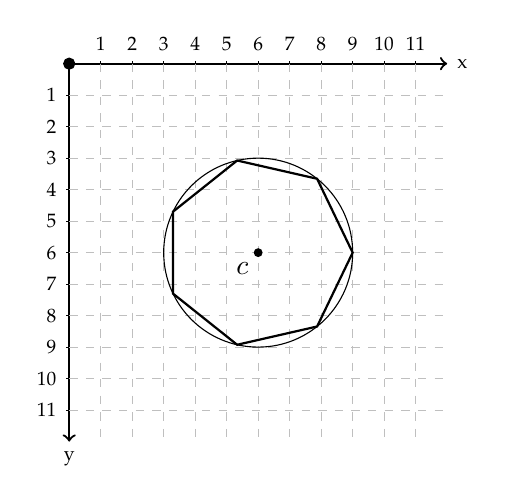
\begin{tikzpicture}
        \begin{scope}[yscale=-1, yshift=-5cm, xshift=5cm, scale=0.4]
            \drawaxesgrid{12}{12}
            % Draw a circle with a dot in the centre
            \draw [thin] (6,6) circle (3);

            % Calculate the vertices of a heptagon (7-sided polygon)
            \foreach \i in {0,1,...,6} {
                    \pgfmathsetmacro{\angle}{360/7*\i}
                    \pgfmathsetmacro{\x}{6 + 3*cos(\angle)}
                    \pgfmathsetmacro{\y}{6 + 3*sin(\angle)}
                    \coordinate (P\i) at (\x,\y);
                }

            % Draw the heptagon
            \draw[thick] (P0) -- (P1) -- (P2) -- (P3) -- (P4) -- (P5) -- (P6) -- cycle;

            \fill (6,6) circle (4pt) node[anchor=north east] {$c$};
        \end{scope}
    \end{tikzpicture}
\end{center}

\subsubsection{Point in Circle Intersection}
To determine if a point lies within a circle, we can calculate the distance
from the point to the center of the circle and compare it to the circle's
radius.

Given a circle with center $c$ and radius $r$, and a point $p$, the distance
between the point and the center is given by:

\begin{equation}
    \begin{aligned}
        d_x & = p.x - c.x                \\
        d_y & = p.y - c.y                \\
        d   & = \sqrt{{d_x}^2 + {d_y}^2}
    \end{aligned}
\end{equation}

If the distance $d$ is less than the radius $r$, the point lies within the
circle.

\begin{center}
    \textit{Point lies within circle if and only if:}\\
    $d < r$
\end{center}

\subsubsection{Bounding Circle Intersection}

To detect if two bounding circles intersect, we must first calculate the
difference between the centers of the two circles. Given two circles with
centers $c_1$ and $c_2$ and radii $r_1$ and $r_2$, the distance between the two
centers is given by:

\begin{equation}
    \begin{aligned}
        d_x & = c_2.x - c_1.x            \\
        d_y & = c_2.y - c_1.y            \\
        d   & = \sqrt{{d_x}^2 + {d_y}^2}
    \end{aligned}
\end{equation}

This formula is derived from the Pythagorean theorem, which states that t he
length of the hypotenuse of a right triangle is given by the square root of the
sum of the squares of the two other sides.

\begin{equation}
    c = \sqrt{a^2 + b^2}
\end{equation}

Once we have the distance between the centers, we can determine if the circles
intersect by comparing this distance to the sum of their radii.

\begin{center}
    \textit{Circles intersect if and only if:}\\
    $d < r_1 + r_2$
\end{center}

\subsubsection{Examples}

\begin{figure}[H]
    \begin{center}
        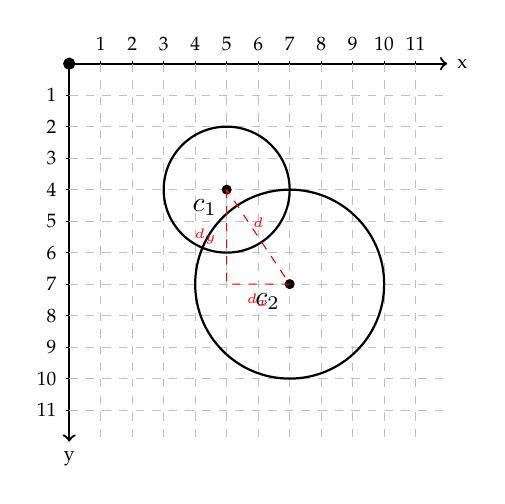
\begin{tikzpicture}
            \begin{scope}[yscale=-1, yshift=-5cm, xshift=5cm, scale=0.4]
                \drawaxesgrid{12}{12}
                % First circle
                \draw [black, thick] (5, 4) circle (2);
                % a point at the center of the first circle
                \filldraw [black] (5, 4) circle (4pt) node[anchor=north east] {$c_1$};
                % Second circle
                \draw [black, thick] (7, 7) circle (3);
                % a point at the center of the second circle
                \filldraw [black] (7, 7) circle (4pt) node[anchor=north east] {$c_2$};

                % Draw triangle representing dx, dy, d
                \draw [red, dashed] (5, 4) -- (5, 7) -- (7, 7) -- cycle;

                % Label dx, dy, d
                \node [red, anchor=east] at (5, 5.5) {\tiny $d_y$};
                \node [red, anchor=north] at (6, 7) {\tiny $d_x$};
                \node [red, anchor=south] at (6, 5.5) {\tiny $d$};

            \end{scope}
        \end{tikzpicture}

        \caption{Bounding Circle Intersection Example}
    \end{center}
\end{figure}

Given two circles with centers $c_1 = (5, 4)$ and $c_2 = (7, 7)$ and radii $r_1
    = 2$ and $r_2 = 3$, use math to determine if the circles intersect.

\subsubsubsection{Mathematical Solution}
First calculate the distance between the two centers:
\begin{equation*}
    \begin{aligned}
        \Delta_x & = 7 - 5 = 2,                                 \\
        \Delta_y & = 7 - 4 = 3,                                 \\
        \Delta   & = \sqrt{2^2 + 3^2} = \sqrt{13} \approx 3.61, \\
    \end{aligned}
\end{equation*}

Now, compare the distance to the sum of the radii:
\begin{equation*}
    \begin{aligned}
        \Delta < r_1 + r_2         & \rightarrow \textnormal{Circles intersect.} \\
        3.61 < 2 + 3               & \rightarrow \textnormal{Circles intersect.} \\
        \textnormal{\textbf{TRUE}} & \rightarrow \textnormal{Circles intersect.} \\
    \end{aligned}
\end{equation*}

Since the distance between the two centers is less than the sum of the radii,
the two circles intersect.

\newpage
\subsubsubsection{Code Solution}
Here is an implementation of the collision detection algorithm in C++:
\vspace{1em}
\begin{mdframed}[linecolor=black!30!white,linewidth=.5pt,extratopheight=3em]
    \begin{lstlisting}[language=C++, aboveskip=3mm,
        belowskip=3mm,
        showstringspaces=false,
        columns=flexible,
        basicstyle={\small\ttfamily},
        numbers=left,
        numberstyle=\tiny\color{gray},
        keywordstyle=\color{blue},
        commentstyle=\color{dkgreen},
        stringstyle=\color{mauve},
        breaklines=true,
        breakatwhitespace=true,
        tabsize=3,
        xleftmargin=1em]
#include "Vec2.h"
#include <cmath>
#include <iostream>

struct Circle {
    Vec2 center;
    float radius;
};

bool checkCollision(const Circle &c1, const Circle &c2) {
    const float dx = c2.center.x - c1.center.x;
    const float dy = c2.center.y - c1.center.y;
    const float distance = std::sqrt(dx * dx + dy * dy);
    const float sumOfRadii = c1.radius + c2.radius;
    const bool collision = distance < sumOfRadii;

    return collision;
}

int main() {
    Circle c1 = {{5, 4}, 2};
    Circle c2 = {{7, 7}, 3};

    if (checkCollision(c1, c2)) {
        std::cout << "Collision detected!" << std::endl;
    } else {
        std::cout << "No collision detected." << std::endl;
    }

    return 0;
}
\end{lstlisting}

\end{mdframed}

\newpage

\section{Axis Aligned Bounding Boxes (AABB)}
In 2D games, objects are often enclosed within rectangles designed to encompass
their width and height, facilitating straightforward collision detection.
Axis-aligned bounding boxes (AABBs) are a specific type of bounding rectangle
used to simplify collision detection between rectangles. Unlike rectangles that
can be oriented in various directions, AABBs are aligned parallel to the $x$
and $y$ axes. This alignment streamlines collision detection algorithms,
allowing us to use simple geometric calculations to determine if two AABBs
intersect.

While AABBs typically encompass the entire width and height of an object, there
are exceptions where the object's image may exceed or be smaller than the
bounding box. This situation is common in animation, where a consistent image
size is used across frames, potentially resulting in sprites that extend beyond
the box's boundaries. Despite these imperfections, which are generally
acceptable in animation, the bounding box is sized to encompass the entire
image.

For example, Mario's standing pose neatly fits within his bounding box, whereas
Megaman's shooting pose extends beyond its boundaries. These variations
highlight how bounding boxes accommodate diverse shapes and sizes in 2D game
design.

\begin{figure}[H]
    \begin{center}
        \begin{tikzpicture}
            \begin{scope}[yscale=-1, yshift=-5cm, xshift=5cm, scale=0.4]
                \drawaxesgrid{18}{9}

                % Adjust the size of Mario to fit within the rectangle
                \node[] (mario) at (4.5, 5)
                {
\includegraphics[width=3.37em, height=4.5em]{mario.png}};

                % Draw the rectangle
                \draw [black, dashed] (3, 3) rectangle (6,7);
                % Label the corners of the rectangle
                \filldraw [black] (3, 3) circle (4pt) node[anchor=north east] {$c_1$};

                \node[] (megaman) at (12, 5)
                {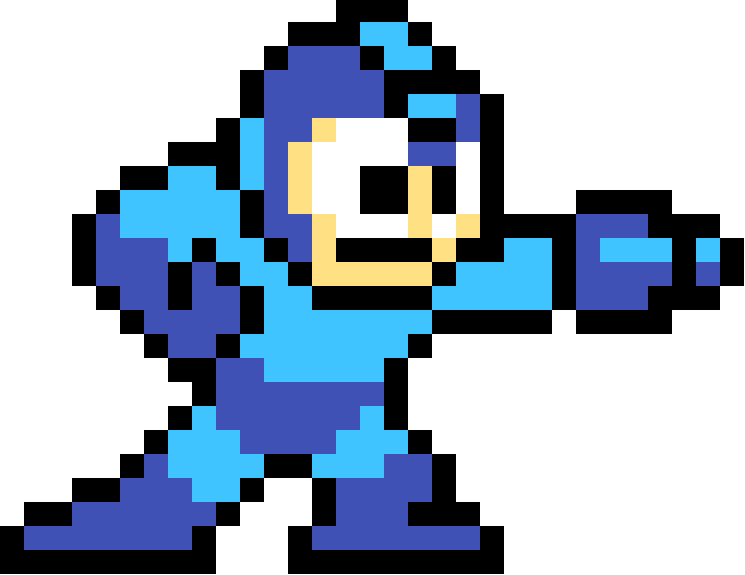
\includegraphics[height=4.6em]{megaman.png}};

                \draw [black, dashed] (10, 3) rectangle (14, 7);
                \filldraw [black] (10, 3) circle (4pt) node[anchor=north east] {$c_2$};

            \end{scope}
        \end{tikzpicture}
    \end{center}

    \caption{Bounding Boxes for Mario and Megaman}
\end{figure}

\subsection{Point and AABB Intersection}

The simplest calculation for AABBs is to check whether a point is inside the
rectangle. Given a point $p$ and a rectangle with corners $c_1$ and $c_2$, we
can determine if the point is inside the rectangle by checking if the point's x
and y coordinates are within the rectangle's x and y coordinates. This is done
by the following formula:
\begin{center}
    \textit{Point $p$ is inside rectangle with corners $c_1$ and $c_2$ if and only if:} \\
    $(p.x > c_1.x) \land (p.x < c_2.x) \land (p.y > c_1.y) \land (p.y < c_2.y)$
\end{center}

If the rectangle is defined by a top left corner $c$, width $w$, and height
$h$, the equation can be modified to:

\begin{center}
    \textit{Point $p$ is inside rectangle with top left corner $c$, width $w$ and height $h$ if and only if:} \\
    $(p.x > c.x) \land (p.x < c.x + w) \land (p.y > c.y) \land (p.y < c.y + h)$
\end{center}
When broken down, the formula is evaluating four conditions:
\begin{multicols}{2}
    \begin{enumerate}
        \item The point's x-coordinate is to the right of the left side of the rectangle.
              \begin{equation*}
                  \begin{aligned}
                      p.x & > c_1.x \\
                      p.x & > c.x
                  \end{aligned}
              \end{equation*}

        \item The point's x-coordinate is to the left of the right side of the rectangle.
              \begin{equation*}
                  \begin{aligned}
                      p.x & < c_2.x   \\
                      p.x & < c.x + w
                  \end{aligned}
              \end{equation*}
    \end{enumerate}
\end{multicols}

\begin{multicols}{2}
    \begin{enumerate}
        \item[3.]The point's y-coordinate is above the bottom side of the rectangle.
        \begin{equation*}
            \begin{aligned}
                p.y & > c_1.y \\
                p.y & > c.y
            \end{aligned}
        \end{equation*}

        \item[4.] The point's y-coordinate is below the top side of the rectangle.
            \begin{equation*}
                \begin{aligned}
                    p.y & < c_2.y   \\
                    p.y & < c.y + h
                \end{aligned}
            \end{equation*}
    \end{enumerate}
\end{multicols}
\newpage

\subsubsection{Example}

\begin{figure}[H]
    \begin{center}
        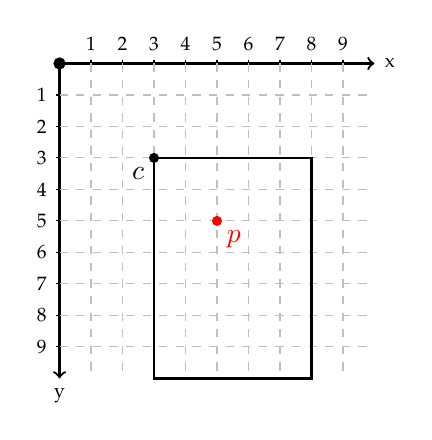
\begin{tikzpicture}
            \begin{scope}[yscale=-1, yshift=-5cm, xshift=5cm, scale=0.4]
                \drawaxesgrid{10}{10}

                % Draw the rectangle
                \draw [black, thick] (3, 3) rectangle (8, 10);
                % Label the corners of the re
                \filldraw [black] (3, 3) circle (4pt) node[anchor=north east] {$c$};

                % Draw the point
                \filldraw [red] (5, 5) circle (4pt) node[anchor=north west] {$p$};

            \end{scope}
        \end{tikzpicture}

        \caption{Rectangle Point Inclusion Example}
    \end{center}
\end{figure}

Given a rectangle with a top left corner $c = (3, 3)$, width $w = 5$, and
height $h = 7$, and a point $p = (5, 5)$, use math to determine if the point
lies within the rectangle.

\subsubsection{Mathematical Solution}
First, calculate the point's x and y coordinates relative to the rectangle's
top left corner:

\begin{equation*}
    \begin{aligned}
        p.x & = 5 - 3 = 2 \\
        p.y & = 5 - 3 = 2
    \end{aligned}
\end{equation*}

Next, check if the point lies within the rectangle:

\begin{equation*}
    \begin{aligned}
        (2 > 0) \land (2 < 5) \land (2 > 0) \land (2 < 7) \rightarrow \text{Point lies within rectangle}. \\
        \textnormal{\textbf{TRUE}} \land \textnormal{\textbf{TRUE}} \land \textnormal{\textbf{TRUE}} \land \textnormal{\textbf{TRUE}} \rightarrow \text{Point lies within rectangle}.
    \end{aligned}
\end{equation*}

Since all four conditions are met, the point lies within the rectangle.

\subsubsection{Code Solution}

Here is an implementation of the point-in-AABB intersection algorithm in C++:

\begin{mdframed}[linecolor=black!30!white,linewidth=.5pt,extratopheight=1em]
    \begin{lstlisting}[language=C++, aboveskip=3mm,
        belowskip=3mm,
        showstringspaces=false,
        columns=flexible,
        basicstyle={\small\ttfamily},
        numbers=left,
        numberstyle=\tiny\color{gray},
        keywordstyle=\color{blue},
        commentstyle=\color{dkgreen},
        stringstyle=\color{mauve},
        breaklines=true,
        breakatwhitespace=true,
        tabsize=3,
        xleftmargin=1em]
#include "Vec2.h"
#include <iostream>

struct AABB {
    Vec2 topLeft;
    float width;
    float height;
};

bool checkPointInAABB(const Vec2 &point, const AABB &rect) {
    const bool pointInAABB = 
        point.x > rect.topLeft.x && point.x < rect.topLeft.x + rect.width &&
        point.y > rect.topLeft.y && point.y < rect.topLeft.y + rect.height;

    return pointInAABB;
}

\end{lstlisting}
\end{mdframed}

\subsection{AABB Intersection}

Determining if two AABBs intersect is a relatively simple task. Given two
AABBs, one may be inclined to check for collision using the point inside AABB
method. However, this is not the most efficient method, as it requires checking
all four corners of one rectangle against the other rectangle. Instead, we can
use an algorithm that detects both horizontal and vertical overlap.

Given two AABBs with top left corners $c_1$ and $c_2$, we can determine if they
overlap horizontally by checking if the right side of the first rectangle is to
the right of the left side of the second rectangle and vice versa. This is done
by the following formula:

\begin{equation}
    \begin{aligned}
         & \textit{Rectangles overlap horizontally if and only if:} \\
         & (c_1.x < c_2.x + c_2.w) \land (c_1.x + c_1.w > c_2.x)
    \end{aligned}
\end{equation}

In a similar manner, we can determine if the rectangles overlap vertically by
checking if the top side of the first rectangle is above the bottom side of the
second rectangle and vice versa. This is done by the following formula:

\begin{equation}
    \begin{aligned}
         & \textit{Rectangles overlap vertically if and only if:} \\
         & (c_1.y < c_2.y + c_2.h) \land (c_1.y + c_1.h > c_2.y)
    \end{aligned}
\end{equation}

Put all together, the AABBs overlap if and only if they overlap both
horizontally and vertically. This is done by the following formula:

\begin{equation}
    % \begin{aligned}
    %      & [(c_1.x < c_2.x + c_2.w) \land (c_1.x + c_1.w > c_2.x)]      \\
    %      & \land[(c_1.y < c_2.y + c_2.h) \land (c_1.y + c_1.h > c_2.y)] \\
    % \end{aligned}
    \begin{aligned}
         & \hspace{1.1em} (c_1.x < c_2.x + c_2.w) \\
         & \land (c_1.x + c_1.w > c_2.x)          \\
         & \land (c_1.y < c_2.y + c_2.h)          \\
         & \land (c_1.y + c_1.h > c_2.y)
    \end{aligned}
\end{equation}

\subsubsection{Example}
\begin{center}
    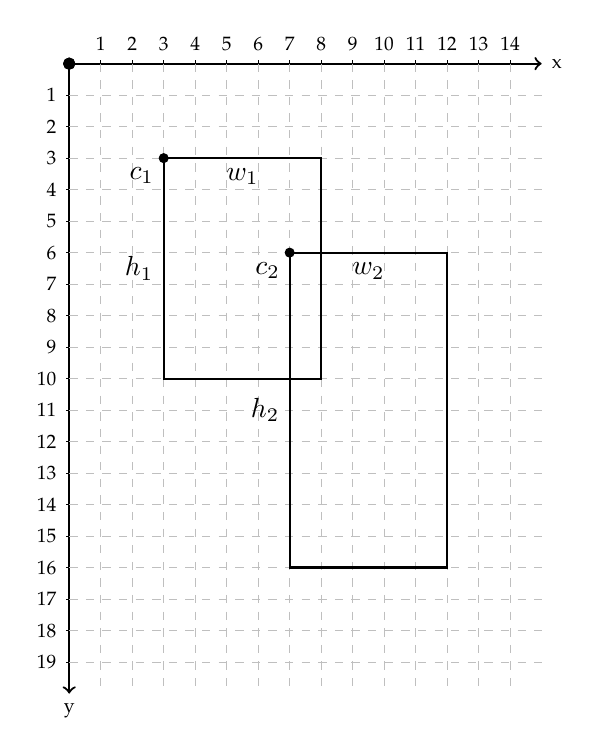
\begin{tikzpicture}
        \begin{scope}[yscale=-1, yshift=-5cm, xshift=5cm, scale=0.4]

            \drawaxesgrid{15}{20}

            % a point at the origin (0, 0) 
            \filldraw [black] (0, 0) circle (5pt) {};

            % First rectangle
            \draw [black, thick] (3, 3) rectangle (8, 10);
            \draw[black, thick, -] (3, 3) -- (8, 3) node[midway, below] {$w_1$};
            \draw[black, thick, -] (3, 3) -- (3, 10) node[midway, left] {$h_1$};
            % a point at the top left corner of the first rectangle

            \filldraw [black] (3, 3) circle (4pt) node[anchor=north east] {$c_1$};
            % Second rectangle
            \draw [black, thick] (7, 6) rectangle (12, 16);
            \draw[black, thick, -] (7, 6) -- (12, 6) node[midway, below] {$w_2$};
            \draw[black, thick, -] (7, 6) -- (7, 16) node[midway, left]
            {$h_2$};
            % a point at the top left corner of the second rectangle
            \filldraw [black] (7, 6) circle (4pt) node[anchor=north east] {$c_2$};

        \end{scope}
    \end{tikzpicture}
\end{center}

Given two rectangles with top left corners $c_1 = (3, 3)$ and $c_2 = (7, 6)$,
widths $w_1 = 5$ and $w_2 = 5$, and heights $h_1 = 7$ and $h_2 = 10$, use math
to determine if the rectangles intersect.

\subsubsection{Mathematical Solution}
First, check if the rectangles overlap horizontally:

\begin{equation*}
    \begin{aligned}
        (3 < 7 + 5) \land (3 + 5 > 7) & \rightarrow \text{Rectangles overlap horizontally}. \\
        \textnormal{\textbf{TRUE}}    & \rightarrow \text{Rectangles overlap horizontally}.
    \end{aligned}
\end{equation*}

Next, check if the rectangles overlap vertically:

\begin{equation*}
    \begin{aligned}
        (3 < 6 + 10) \land (3 + 7 > 6) & \rightarrow \text{Rectangles overlap vertically}. \\
        \textnormal{\textbf{TRUE}}     & \rightarrow \text{Rectangles overlap vertically}.
    \end{aligned}
\end{equation*}

Since the rectangles overlap both horizontally and vertically, they intersect.

\subsubsection{Code Solution}

Here is an implementation of the AABB intersection algorithm in C++:

\begin{mdframed}[linecolor=black!30!white,linewidth=.5pt,extratopheight=1em]
    \begin{lstlisting}[language=C++, aboveskip=3mm,
        belowskip=3mm,
        showstringspaces=false,
        columns=flexible,
        basicstyle={\small\ttfamily},
        numbers=left,
        numberstyle=\tiny\color{gray},
        keywordstyle=\color{blue},
        commentstyle=\color{dkgreen},
        stringstyle=\color{mauve},
        breaklines=true,
        breakatwhitespace=true,
        tabsize=3,
        xleftmargin=1em]

#include "Vec2.h"

struct AABB {
    Vec2 topLeft;
    float width;
    float height;
};

bool checkAABBIntersection(const AABB &a, const AABB &b) {
    const bool horizontalOverlap = 
        a.topLeft.x < b.topLeft.x + b.width && a.topLeft.x + a.width > b.topLeft.x;
    const bool verticalOverlap = 
        a.topLeft.y < b.topLeft.y + b.height && a.topLeft.y + a.height > b.topLeft.y;

    const bool AABBIntersects = horizontalOverlap && verticalOverlap;

    return AABBIntersects;
}

int main() {
    AABB a = {{3, 3}, 5, 7};
    AABB b = {{7, 6}, 5, 10};

    if (checkAABBIntersection(a, b)) {
        std::cout << "AABBs intersect." << std::endl;
    } else {
        std::cout << "AABBs do not intersect." << std::endl;
    }

    return 0;
}

\end{lstlisting}
\end{mdframed}

It is important to note that the above formula can only check whether or nor
not two AABBs intersect. It does not provide information on how much they
intersect.

To determine the overlap, we can use a calculation that takes a center point
and the width and height of the bounding box. This is done as follows:

Given two AABBs with centers $c_1$ and $c_2$, widths $w_1$ and $w_2$, and
heights $h_1$ and $h_2$,

\begin{equation}
    \begin{aligned}
        \Delta                        & = \left\{ \left| c_1.x - c_2.x \right| , \left| c_1.y - c_2.y \right| \right\}                                                                                     \\
        O                             & = \left\{ \left[ \left( \frac{w_1}{2} + \frac{w_2}{2} \right) - \Delta_x \right] , \left[ \left( \frac{h_1}{2} + \frac{h_2}{2} \right) - \Delta_y \right] \right\} \\
        ( O_x > 0 ) \land ( O_y > 0 ) & \rightarrow \text{AABBs intersect}
    \end{aligned}
\end{equation}

In this formula, the vector $\Delta$ represents the absolute difference between
the center coordinates of the two AABBs along the $x$ and $y$ axes.

The vector $O$ represents the overlap between the two AABBs along the $x$ and
$y$ axes. The overlap along each axis is calculated by subtracting the
difference between the centers from the sum of the half-widths (for the $x$
axis) or half heights (for the $y$ axis) of the two AABBs.

\subsubsection{Example}

Given two AABBs with centers $c_1 = (3, 3)$ and $c_2 = (7, 6)$, widths $w_1 =
    5$ and $w_2 = 5$, and heights $h_1 = 7$ and $h_2 = 10$, use math to determine
the overlap between the two AABBs.

\subsubsection{Mathematical Solution}

First, calculate the absolute difference between the centers of the two AABBs:

\begin{equation*}
    \begin{aligned}
        \Delta_x & = \left| 3 - 7 \right| = 4 \\
        \Delta_y & = \left| 3 - 6 \right| = 3
    \end{aligned}
\end{equation*}

Next, calculate the overlap between the two AABBs along the $x$ and $y$ axes:

\begin{equation*}
    \begin{aligned}
        O_x & = \left( \frac{5}{2} + \frac{5}{2} \right) - 4 = 1    \\
        O_y & = \left( \frac{7}{2} + \frac{10}{2} \right) - 3 = 3.5
    \end{aligned}
\end{equation*}

Finally, check if the AABBs intersect:

\begin{equation*}
    \begin{aligned}
        (1 > 0) \land (3.5 > 0)    & \rightarrow \text{AABBs intersect} \\
        \textnormal{\textbf{TRUE}} & \rightarrow \text{AABBs intersect}
    \end{aligned}
\end{equation*}

Since the overlap along both axes is positive, the AABBs intersect.

\subsubsection{Code Solution}

Here is an implementation of the AABB overlap algorithm in C++:

\begin{mdframed}[linecolor=black!30!white,linewidth=.5pt,extratopheight=1em]
    \begin{lstlisting}[language=C++, aboveskip=3mm,
        belowskip=3mm,
        showstringspaces=false,
        columns=flexible,
        basicstyle={\small\ttfamily},
        numbers=left,
        numberstyle=\tiny\color{gray},
        keywordstyle=\color{blue},
        commentstyle=\color{dkgreen},
        stringstyle=\color{mauve},
        breaklines=true,
        breakatwhitespace=true,
        tabsize=3,
        xleftmargin=1em]
#include "Vec2.h"
#include <iostream>

struct AABB {
    Vec2 center;
    float width;
    float height;
};

bool checkAABBOverlap(const AABB &a, const AABB &b) {
    const Vec2 delta = {std::abs(a.center.x - b.center.x), std::abs(a.center.y - b.center.y)};
    const Vec2 overlap = {((a.width / 2) + (b.width / 2)) - delta.x, ((a.height / 2) + (b.height / 2)) - delta.y};

    const bool overlapX = overlap.x > 0;
    const bool overlapY = overlap.y > 0;

    const bool AABBsIntersect = overlapX && overlapY;

    return AABBsIntersect;
}

int main() {
    AABB a = {{3, 3}, 5, 7};
    AABB b = {{7, 6}, 5, 10};

    if (checkAABBOverlap(a, b)) {
        std::cout << "AABBs intersect." << std::endl;
    } else {
        std::cout << "AABBs do not intersect." << std::endl;
    }

    return 0;
}
\end{lstlisting}
\end{mdframed}



\chapter{Collision Resolution}
\lipsum[1-4]

\section*{Appendix}

The following code snippets are implementations of the \texttt{Vec2} class in
C++. The \texttt{Vec2} class is a simple two-dimensional vector class that
provides basic vector operations such as addition, subtraction, multiplication,
and division. The class is used in this document for various collision
detection and resolution algorithms.

\subsection*{Vec2.h}
\vspace{1em}
\begin{mdframed}[linecolor=black!30!white,linewidth=.5pt,extratopheight=1em]
    \lstinputlisting[
        language=C++,
        aboveskip=3mm,
        belowskip=3mm,
        showstringspaces=false,
        columns=flexible,
        basicstyle={\small\ttfamily},
        numbers=left,
        numberstyle=\tiny\color{gray},
        keywordstyle=\color{blue},
        commentstyle=\color{dkgreen},
        stringstyle=\color{mauve},
        breaklines=true,
        breakatwhitespace=true,
        tabsize=3,
        xleftmargin=1em
    ]{code-examples/Vec2.h}
\end{mdframed}

\subsection*{Vec2.cpp}
\vspace{1em}
\begin{mdframed}[linecolor=black!30!white,linewidth=.5pt,extratopheight=1em]
    \lstinputlisting[
        language=C++,
        aboveskip=3mm,
        belowskip=3mm,
        showstringspaces=false,
        columns=flexible,
        basicstyle={\small\ttfamily},
        numbers=left,
        numberstyle=\tiny\color{gray},
        keywordstyle=\color{blue},
        commentstyle=\color{dkgreen},
        stringstyle=\color{mauve},
        breaklines=true,
        breakatwhitespace=true,
        tabsize=3,
        xleftmargin=1em
    ]{code-examples/Vec2.cpp}
\end{mdframed}
\end{document}
